\documentclass[]{aiaa-tc}% insert '[draft]' option to show overfull boxes

\usepackage{mathtools,amssymb}

\usepackage{gensymb}

\usepackage{array,multirow,rotating}
\usepackage{ifthen}
\usepackage{graphicx}
\usepackage{varioref}%  smart page, figure, table, and equation referencing
\usepackage{wrapfig}%   wrap figures/tables in text (i.e., Di Vinci style)
\usepackage{threeparttable}% tables with footnotes
\usepackage{dcolumn}%   decimal-aligned tabular math columns
 \newcolumntype{d}{D{.}{.}{-1}}
\usepackage{nomencl}%   nomenclature generation via makeindex
\usepackage{makeidx}
 \makenomenclature
\usepackage{subfigure}% subcaptions for subfigures
\usepackage{subfigmat}% matrices of similar subfigures, aka small mulitples
\usepackage{fancyvrb}%  extended verbatim environments
 \fvset{fontsize=\footnotesize,xleftmargin=2em}
\usepackage{lettrine}%  dropped capital letter at beginning of paragraph
%\usepackage[dvips]{dropping}% alternative dropped capital package
\usepackage{hyperref}%  hyperlinks [must be loaded after dropping]

\hypersetup{
  colorlinks   = true, %Colours links instead of ugly boxes
  urlcolor     = black, %Colour for external hyperlinks
  linkcolor    = black, %Colour of internal links
  citecolor   = black %Colour of citations
}

\graphicspath{ {./images/} }

\title{AIAA Latex Template}

\author{
 Metin F. Ozcan\thanks{Graduate Research Assistant, Aerospace Systems Design Laboratory (ASDL), 275 Ferst Drive NW, Atlanta, GA 30332-0150, and AIAA Student Member.}
 \ , Imon Chakraborty\footnotemark[1]
 \ , and Dimitri N. Mavris\thanks{Boeing Regents Professor of Advanced Aerospace Systems Analysis, Director at ASDL, and AIAA Fellow.}  \\
 {\normalsize\itshape
  School of Aerospace Engineering, Georgia Institute of Technology, Atlanta, GA, 30332}
}

% Data used by 'handcarry' option
\AIAApapernumber{YEAR-NUMBER}
\AIAAconference{Conference Name, Date, and Location}
\AIAAcopyright{\AIAAcopyrightD{YEAR}}

% Define commands to assure consistent treatment throughout document
\newcommand{\eqnref}[1]{(\ref{#1})}
\newcommand{\class}[1]{\texttt{#1}}
\newcommand{\package}[1]{\texttt{#1}}
\newcommand{\file}[1]{\texttt{#1}}
\newcommand{\BibTeX}{\textsc{Bib}\TeX}

\newcommand{\superscript}[1]{\ensuremath{^{\textnormal{#1}}}}
\newcommand{\subscript}[1]{\ensuremath{_{\textnormal{#1}}}}

%\RequirePackage{ifthen}
%\renewcommand{\nomgroup}[1]{%
%\ifthenelse{\equal{#1}{G}}{\item[\textbf{Greek Symbols}]}{
%\ifthenelse{\equal{#1}{S}}{\item[\textbf{Subscripts}]}{}}}

\begin{document}

\nomenclature{$TONE$}{The only nomenclature entry, Units go here}

\maketitle

\begin{abstract}

Fan variable area nozzles (FVAN) can provide several benefits, such as improving propulsive efficiency, reducing jet noise, increasing fan surge margin, and controlling fan flutter margin, by changing the FVAN area as a function of the current operating condition.  For example, the top of climb flight condition requires a smaller FVAN area whereas take-off requires a larger FVAN area. When analyzing the performance at these steady-state flight conditions, the aforementioned benefits are observed.  However, the gas turbine must operate one steady-state condition to another safely throughout the mission to realize these benefits. 

During a transition from one steady-state condition to another, FVAN must respond in concert with shaft dynamics for performance and safety. If FVAN doesn't respond in accordance with the shaft dynamics, either thrust lapse or stall can occur at different flight conditions. The response time of FVAN depends strongly on actuator dynamics. Lighter actuators with shape memory alloys (SMA) were proposed instead of heavy and complex conventional hydraulic actuators to reduce the fuel burn penalty due to actuator weight when FVAN is on-board. The SMA actuators are more flexible and lighter, but also respond slower than the hydraulic actuators. Therefore, a gas turbine controller must compensate for the slower SMA actuators while controlling either one variable (fuel flow rate with FVAN schedule) or two variables (fuel flow rate and FVAN). This study aims to evaluate how current SMA actuators perform. %If current SMA actuators fail, how slow SMA actuators are acceptable will be determined.  %Do we need this last sentence?

The SMA actuators will be represented by a first order lag with representative time constant values selected from previous work on SMA actuators.  Using a gas turbine model in the small single aisle thrust class, closed-loop controllers will be developed for the cases where FVAN runs with a schedule and when a closed-loop controller directly regulates the FVAN area. Gas turbine transient performance for the two FVAN cases will be analyzed based on thrust lapse and stall margin. A signal with a series of steps, chops, and ramps will be used to test the two developed controllers. If the gas turbine cannot reach 98\% of maximum thrust in less than five seconds (FAA requirement) or keep a safe stall margin throughout the transient operation, the time constant will be reduced to determine the SMA actuator response required to meet the performance and safety requirements.
%A first order lag will represent the SMA actuators and the representative time constant values are selected from the literature on the SMA actuators. Using a gas turbine model in small single aisle thrust class, controllers will be developed for the cases where FVAN runs with a schedule or a controller changes FVAN area directly. Gas turbine transient performance for the two FVAN cases will be analyzed based on thrust lapse and stall margin. A signal with a series of steps, chops, and ramps will be used to test the two developed controllers. If the gas turbine cannot reach 98\% of maximum thrust in less than five seconds (FAA requirement) or keep a safe stall margin throughout the transient operation, the time constant will be reduced to observe how fast the SMA actuator needs to be for performance and safety.

\end{abstract}

\printnomenclature % creates nomenclature section produced by MakeIndex

\section{Introduction}

\lettrine[nindent=0pt]{V}{ariable} geometry components promise improvements in gas turbine performance and safety. However, the improvements come with more complexity in addition to a necessary trade-off study due to the additional actuator system. Fan variable area nozzle (FVAN) is an example for the improvements, increase in complexity, and trade-off. FVAN can improve propulsive efficiency, reduce jet noise, increase fan surge margin, and control fan flutter margin. On the other hand, the FVAN actuator system can reduce the efficiency increase due to its extra weight and the additional control variable - variable nozzle area - complicates the control system unless the variable nozzle area is scheduled. Scheduling does not provide better performance or safety than controlling directly. 

The cost and benefit analysis for FVAN has considered only steady state analysis so far. What the FVAN area should be at different steady state points can be determined to realize the mentioned benefits. For example, top of climb requires a smaller FVAN area whereas take-off requires a larger FVAN area. However, the gas turbine must switch from one steady state condition to another safely throughout the mission. During a transition from one steady state condition to another, FVAN must respond in concert with shaft dynamics for performance and safety. If FVAN doesn't respond in accordance with shaft dynamics, either thrust lapse or stall can occur at different flight conditions. 

How fast FVAN responds, depends strongly on how fast the actuator is. Lighter actuators with shape memory alloys (SMA) \cite{Mabe:2008,Mabe:2008:Paris} were proposed instead of heavy and complex conventional hydraulic actuators to reduce the fuel burn penalty due to actuator weight when FVAN is on-board. The SMA actuators are more flexible, lighter and slower than hydraulic actuators \cite{Rey:2001,Barooah:2002,Song:2007}. In addition, FVAN is a challenging application for SMA because above a certain temperature SMA material properties transition. Consequently, SMA actuator placement is important for FVAN application.  

Before determining where to place the SMA actuator, a gas turbine controller must compensate for the slower SMA actuators while controlling either one variable (fuel flow rate with FVAN schedule) or two variables (fuel flow rate and FVAN). This study aims to evaluate how current SMA actuators perform with their dynamic characters in transient operation. If current SMA actuators do not meet the performance and safety requirements, the second aim is to determine how fast SMA dynamics must be to meet the requirements.

The paper is divided into three parts. First, the gas turbine engine model used in this study will be presented. Particular details about FVAN modeling will be given in addition to multi-design point cycle design values. After covering the gas turbine model, the controller development processes for scheduled and controlled dynamic FVAN will be discussed. Finally, the results for the transient operation with the dynamic FVAN will be shown and analyzed. 

\section{The section that follows the introduction}
Content for this section goes here.

% Two figures side by side
\begin{figure}[!htb]
\begin{minipage}[b]{0.5\linewidth}
\begin{center}
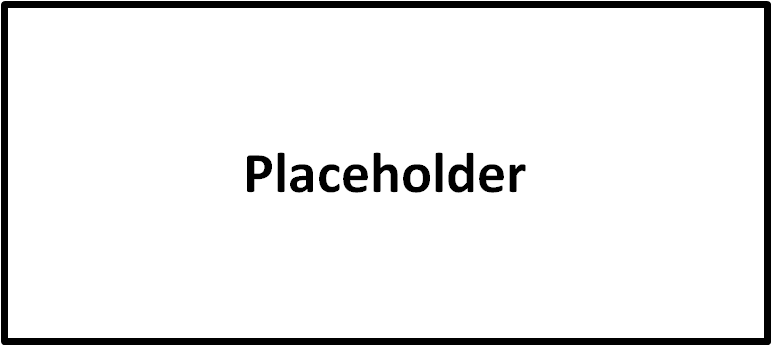
\includegraphics[width=\textwidth,height=\textheight,keepaspectratio]{placeholder.png}
\end{center}
\end{minipage}
\hspace{0.5cm}
\begin{minipage}[b]{0.5\linewidth}
\begin{center}
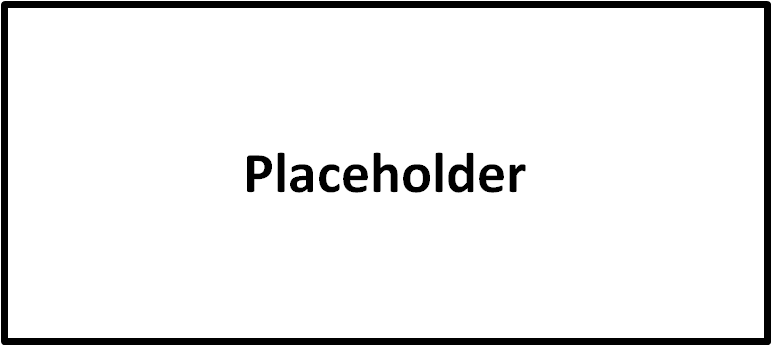
\includegraphics[width=\textwidth,height=\textheight,keepaspectratio]{placeholder.png}
\end{center}
\end{minipage}
\caption{Two placeholder figures side by side}
\label{fig:side_by_side_placeholders}
\end{figure}

\section{Just another section}

\autoref{eq:example_equation} is the first equation in this document.

% Example equation
\begin{equation} \label{eq:example_equation}
p(z)\approx \frac{k}{NV}
\end{equation}

You can also write down a group of equations as in \autoref{eq:example_eqn_group}.

% Example equation array
\begin{eqnarray}
\label{eq:example_eqn_group}
c_{D} = \frac{2\pi^{D/2}}{D \cdot \Gamma(D/2)} \\
\Gamma(t) = \int_{0}^{\infty} x^{t} \mathrm{e}^{-x} \frac{\mathrm{d}x}{x} \nonumber
\end{eqnarray}

\section{A section with a table}

After introducing figures and equations, it is time to introduce a table as in \autoref{tbl:example}.

% Example table
\begin{table}[!htb]
\caption{Example table}
\label{tbl:example}
\begin{center}
\begin{tabular}{|c|c|}
\hline
\textbf{First column} & \textbf{Second column} \\ \hline
First item & 1.5 \\ \hline
Second item & 0.89 \\ \hline
Third item & 2650 \\ \hline
\end{tabular}
\end{center}
\end{table}

The simple table in \autoref{tbl:example} is followed by a more involved example in \autoref{tbl:complex_example}.

\begin{table}[!htb]
\caption{Evaluation results for the input signals selected from the literature}
\label{tbl:complex_example}
\begin{center}
\begin{tabular}{|c|c|c|c|c|}
\cline{2-5}
\multicolumn{1}{c|}{} & \multicolumn{4}{c|}{Density Estimation Evaluation Points} \\
\cline{2-5}
\multicolumn{1}{c|}{} & Boundary & Interior & Equilibrium & Overall \\ \hline
Steps with multisine & 0.0577 & 0.0398 & 0.0206 & 0.0456 \\ \hline
Triangular wave & 0.1525 & 0.0751 & 0.1069 & 0.1009 \\ \hline
Step and chop series & 0.0063 & 0.0564 & 0.0464 & 0.0397 \\ \hline
\end{tabular}
\end{center}
\end{table}

\section{Conclusion}

Conclusion goes here.

% produces the bibliography section when processed by BibTeX
\bibliography{reference_database}
\bibliographystyle{aiaa}

\end{document} 